%\begin{figure*}[ht]
%\begin{center}
%   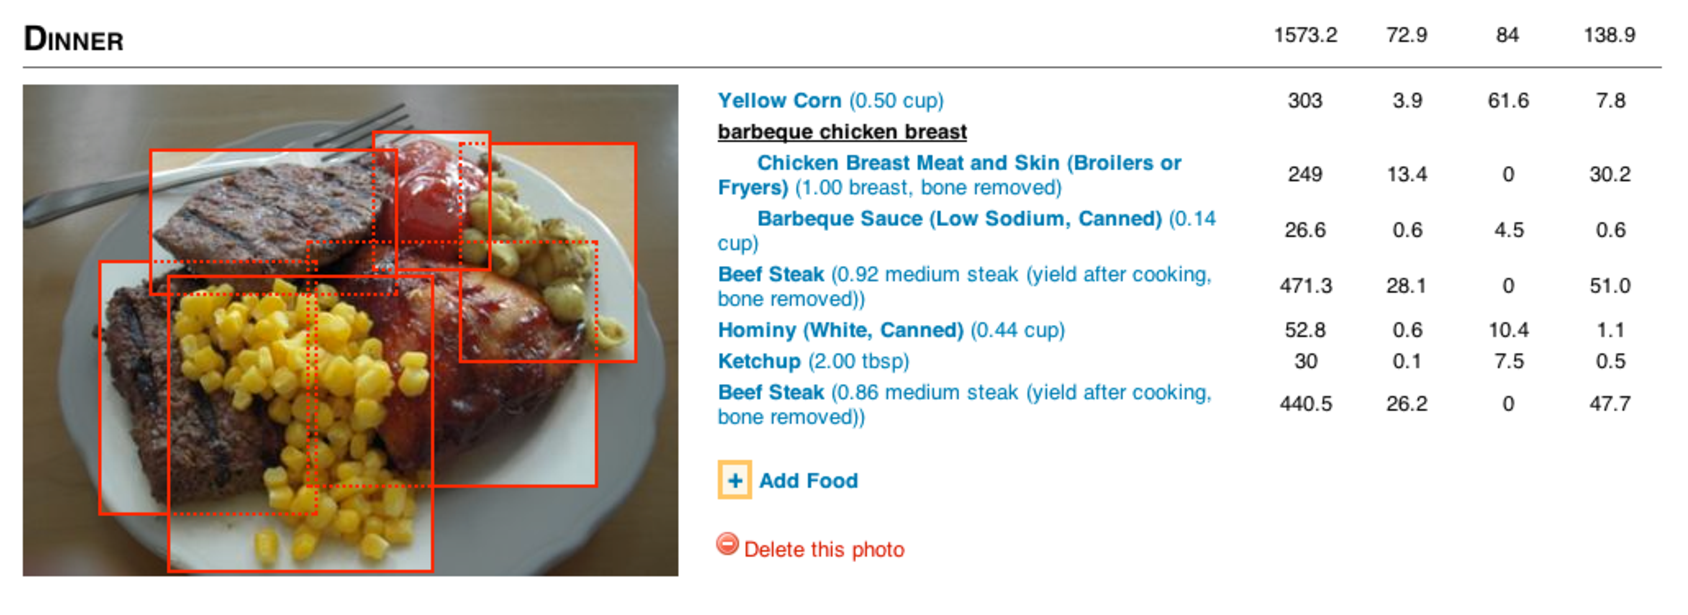
\includegraphics[width=\linewidth]{figs/ui.pdf}
%   \caption{The PlateMate user interface.  Users upload photographs of their meals, which are processed through Mechanical Turk to produce a list of foods, serving sizes, and nutrition information.}
%   \label{fig:ui}
%\end{center}
%\end{figure*}


\section{PLATEMATE}
PlateMate allows users to upload food photographs and receive
nutrition estimates within a few hours. \newcontent{The estimates 
  consist of a list of foods in the photograph, with
  associated measurements of serving size, calories, fat,
  carbohydrates, and protein for each food item. The information is
  displayed to the user via the user interface shown in
  Figure~\ref{fig:ui}.}

Estimates are generated from a
series of tasks on Amazon Mechanical Turk. Crowdsourcing nutritional
analysis presents several challenges in interface and workflow
design. \newcontent{First, Turkers are inexperienced, and may thus
  produce unreliable estimates. Second, most Mechanical Turk tasks are
  simple, and Turkers may be unaccustomed to performing complex
  operations like nutritional analysis if presented as a single,
  complex task. Finally, any individual Turker may be biased in their
  estimates or have trouble recognizing certain foods contained in a
  photograph, making it necessary to select from or combine the
  outputs of multiple workers.}
%As Turkers are
%inexperienced and their estimates may thus be unreliable,
% because Turkers are inexperienced and may produce unreliable
%estimates.  Most tasks on They are suited to performing very small
%tasks rather than complex operations like nutrition analysis.

To best design a workflow for crowdsourcing nutritional analysis, we
started by observing a dietitian as she determined nutritional data
from several photographs.  Her process consisted of three distinct
steps: identifying foods in each image, estimating their portions, and
then calculating the corresponding nutrition data. The final step can
be fully computerized, but PlateMate implements the first two with
crowdsourcing. Following Soylent~\cite{bernstein2010soylent}, we also
add an input decomposition stage at the start to parallelize work.

The result is a workflow with three major stages, shown in
Figure~\ref{fig:system}. \emph{Tag} takes photos and labels them with
boxes drawn around distinct foods on a plate.  \emph{Identify} matches
each box to one or more foods in a commercial nutrition database.
\emph{Measure} returns portion estimates for each identified food.
%Each stage routes work through one or more Human Intelligence Tasks
%(HITs). Generally, an initial task is assigned to several Turkers who
%provide potentially conflicting responses. These responses are then
%resolved into a single answer through some combination of algorithmic
%decisions and further human review.  The design of each stage and its
%component HITs is described in detail below.

\begin{figure*}[t]
\begin{center}
   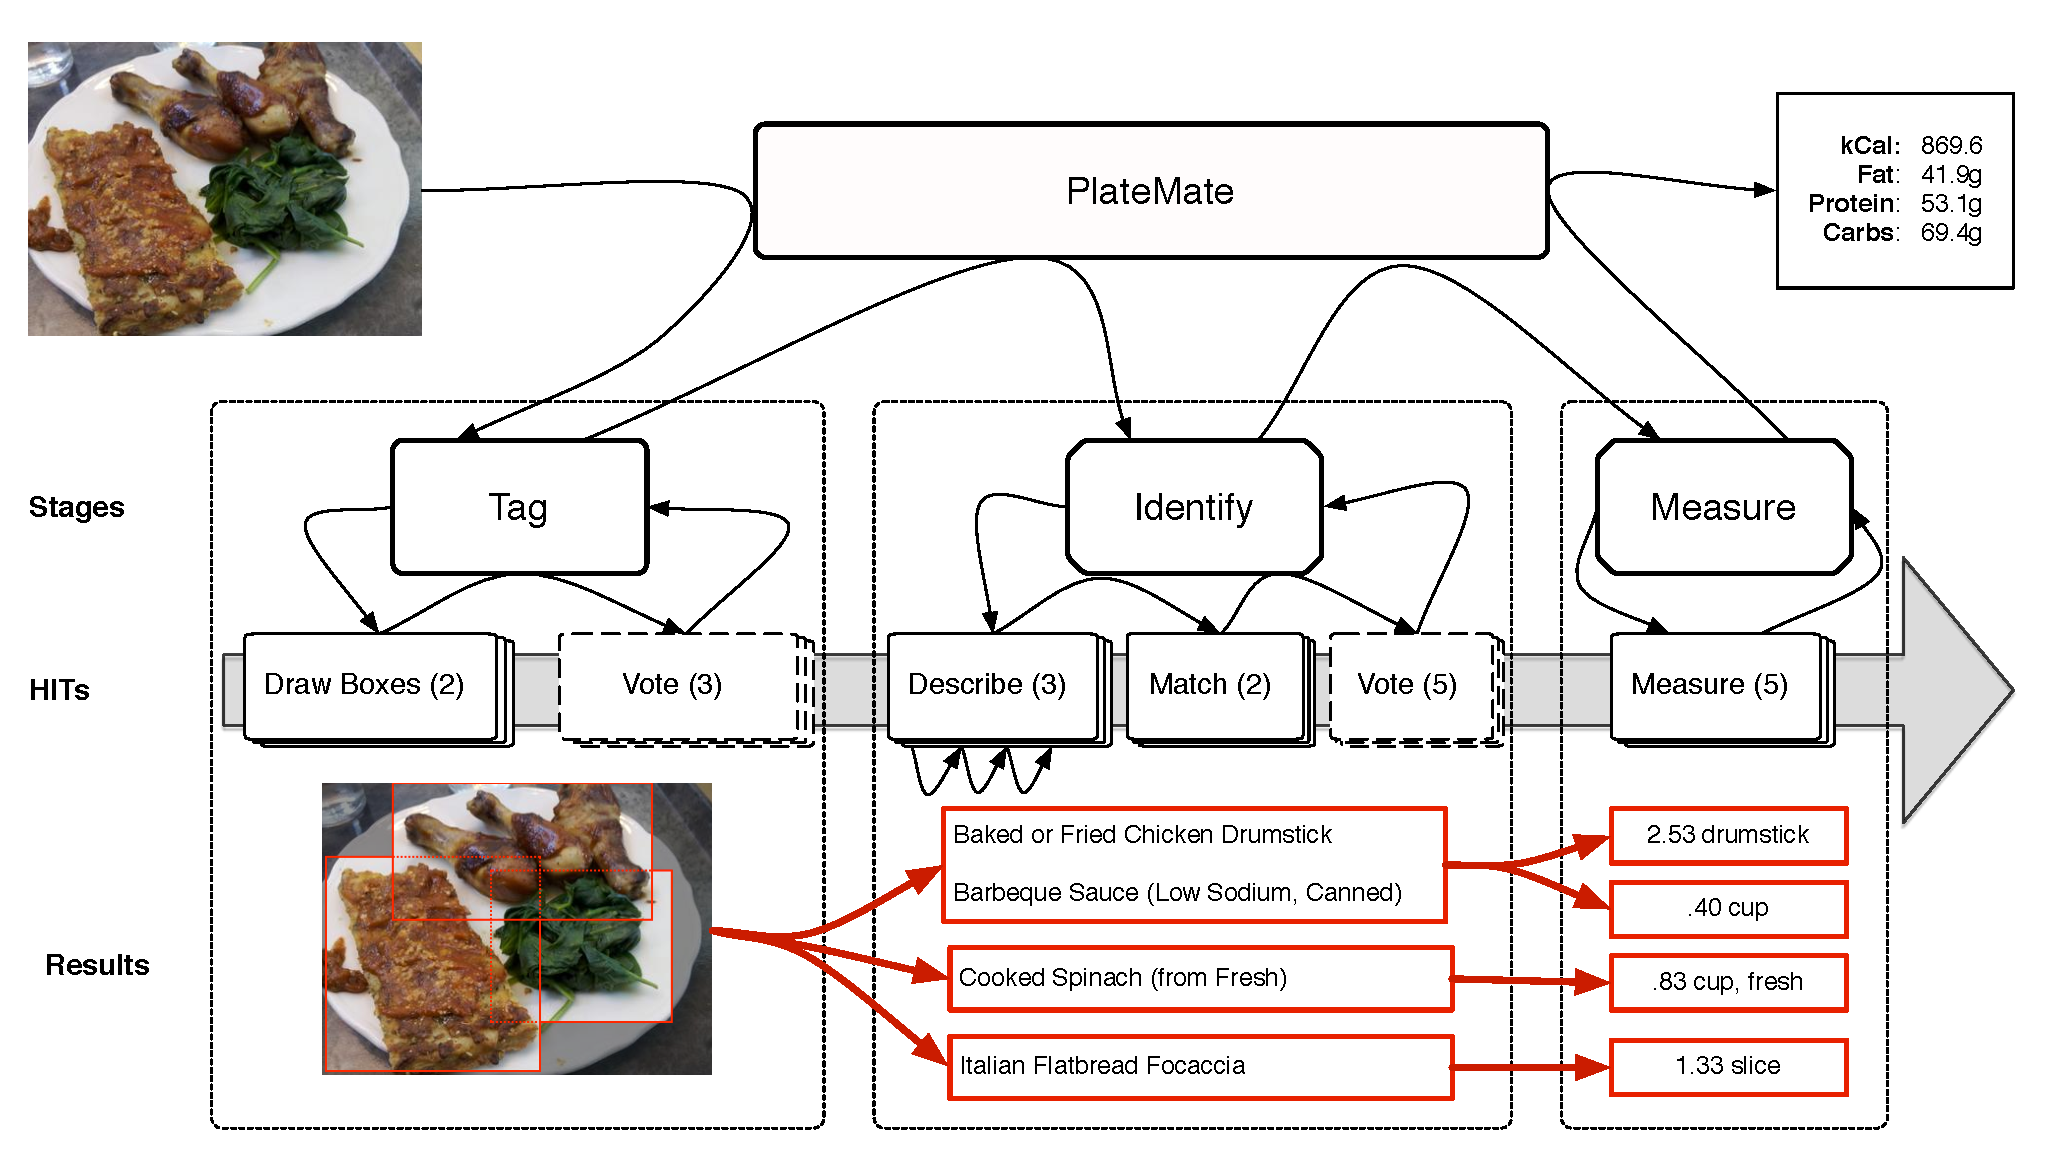
\includegraphics[width=\linewidth]{figs/diagram.pdf}
   \caption{The PlateMate system. Work travels between stages and
     Human Intelligence Tasks (HITs) along the black arrows, starting
     from the input on the left and concluding with the output on the
     right. The system takes submitted photos and creates Tag tasks to
     annotate these photos with boxes.  Each box becomes the input to
     a series of Identify tasks which end with a list of foods from a
     commercial food database.  Each individual food is then input to
     a Measure task, which produces a unit and amount.  Dashed boxes
     represent optional stages, which may be skipped during routing.}
   \label{fig:system}
\end{center}
\end{figure*}

\subsection{Step 1: Tag}
%\emph{Input: one photograph}\\
%\emph{Output: many boxes}

The goal of the Tag stage is to find every food item in a
photograph. One picture may depict several plates, and each plate
might contain several distinct foods. Tag discovers these foods and
distinguishes them by drawing a rectangle around each. The result is a
group of boxes overlaid on the picture. Each box corresponds to a
single food item, like a sandwich.
%These items might be composite foods, like sandwiches, which are comprised of many intuitively related parts, like bread and turkey.

This step has the same benefits as the Find stage in Soylent's
Find-Fix-Verify pattern~\cite{bernstein2010soylent}. Results can be
surfaced more naturally in the user interface, and this makes
estimates easier to understand and correct. Parallel work can also be
combined more carefully, since we know which identifications describe
each pictured food. Finally, the Tag step encourages completeness,
preventing ``Lazy Turkers'' from ignoring or forgetting to match
certain foods.

\subsubsection{Drawing Boxes} 
Tag's first Human Interactive Task (HIT) asks workers to draw boxes
around each food in the picture. Workers need cultural background
knowledge to understand how foods on a plate fit together. Pure
computer vision can detect edges and boundaries, but it cannot
recognize that an open-faced hamburger with half of the bun off to the
side is in fact one item. The HIT relies on Turkers' general
intuition about food items, and provides examples of sandwiches,
salads, and pasta with vegetables as appropriate items.

\subsubsection{Similarity Comparison and Voting} 
Two Turkers are asked to tag each photo, and a combination of machine
and human computation is used to select the better box group.  Once
both assignments are completed, they are algorithmically compared in
the number, size, and position of boxes. If the two groups are
sufficiently similar, one is picked at random as the final answer.

If the box groups differ significantly, three additional Turkers are
shown each set overlaid on the photo and asked to select the better
option, using similar guidelines.  The box group receiving more votes
is returned as the final result.

\subsection{Step 2: Identify}
%\emph{Input: one box}\\
%\emph{Output: many foods}

The Identify step matches a tagged box to one or more food entries in
a commercial nutrition database. While each box output from Tag should
only contain one food, some composite items do not exist in the
database. For example, if ``ham and cheese sandwich'' is missing,
Identify should choose ``wheat bread,'' ``sliced ham,'' and ``American
cheese.''

There are two main challenges in this stage. Identifications must be
correct, and when several correct identifications exist, the most
compact one should be used in order to simplify measurement and eventual
presentation of data to end users.

In an initial pilot study, Identify was performed in a single
HIT. Workers used an autocomplete text input to list each food in the
box.  Their answers were frequently incorrect or incomplete. Workers
appeared to type a one-word description of the picture, like
``chicken,'' and then select the first option regardless of how
closely it fit. Like the ``Lazy Turkers''
in~\cite{bernstein2010soylent}, they performed the minimal work
necessary to get paid and nothing more.

These problems also occurred because the interface asked Turkers to
perform two conceptually different tasks sequentially but only produce
one final output. Turkers first had to identify the food in their own
minds, and then locate the corresponding entries in the database. To
correct for this, we developed a workflow that contained two simpler
HITs. The first asks workers to describe the food in their own
words. The second asks them to match this description to items in the
database.

\subsubsection{Describing Items} In this HIT, Turkers see a box on a photo. One question asks ``What is this food?'', requesting one-line descriptions like ``pepperoni pizza`` or ``salad with chicken.'' Another asks ``What is it made of?'', providing a free-form text field where workers can list component parts. For simple foods like broccoli these fields will be identical, but for composite foods the fields should have different answers that are each useful.

Following successful prior experiments in describing
images~\cite{little2010turkit}, we made this step
\emph{iterative}. One worker starts from blank boxes. Her answer
becomes input to another HIT, where the next Turker is asked to
improve on it by correcting mistakes and adding detail. This process
is well-suited to the ``Eager Beavers'' of
\cite{bernstein2010soylent}, who provide minute details and list many
possibilities. It also handles ``Lazy Turkers'' well, since terse
descriptions are progressively expanded.

\subsubsection{Matching Foods} 
After three iterations, the output of the Describe task is fed into a
Match HIT. Here, workers see the photo and the final
descriptions. They are asked to select the best entry or set of
entries in the database to match the box, with the descriptions as a
suggestion for what to search. Workers first attempt to locate the
description of the box as a whole in the database. If they find no
good match, they search for each part. For example, workers should
first search for ``salad with chicken and tomatoes.'' If this fails,
they should look for ``chicken breast'', ``romaine lettuce'', and
``cherry tomatoes.''

The search interface is modified from a standard autocomplete.  Search
results display below the input box, but the keyboard cannot be used
for quick selection. Turkers must use the mouse to click the correct
items to add. The interface also makes it clearer that multiple items
can be selected through several searches.  These changes negate the
instinct of ``Lazy Turkers'' from the pilot study to select the first
item they see.

This decomposition makes each step manageable for Turkers moving
rapidly through HITs.  The results of the Describe step are not
necessary for the end goal of calculating nutrition information, but the 
generated descriptions reduce the mental work required for the Match
step.  We can then ask Turkers working on Match HITs to find
the simplest representation in the database, using the Describe
results as a guide.

\subsubsection{Agreement Detection and Voting} 
Two workers are asked to complete each Match HIT. If each returns a
list pointing to the exact same item or items in the food database,
then that list is used.  Otherwise, five workers complete a Vote HIT
to decide between them.

\subsection{Step 3: Measure}

The Measure step produces an estimated portion size for each food
matched in Identify. Following this stage, the nutrition data for a
photo can be calculated by multiplying the per-unit nutrition
breakdown from the food database with the estimated measurement for
each identified food.

Measure uses only one HIT, which shows Turkers a photo with a box
highlighted along with the name of one food in that box. They are
asked to first select a measurement unit and then provide a numeric
estimate in terms of that unit. The units provided by the food
database are specific to each food. ``Pepperoni pizza'' includes
options like ``slice, large'' or ``whole pie, medium,'' while ``white
rice, cooked'' uses cups or ounces.

Measurement is considered the most difficult step of this process for
amateurs~\cite{martin2009novel}, so the Measure stage uses a number of
techniques to produce accurate results. Presenting multiple
measurement options is helpful, since many of these only require
counting rather than estimating a weight or volume. For example, it is
much easier to count florets than to estimate grams of broccoli.

Not every food can be measured by counting.  To help in cases where
weight or volume estimates are necessary, HITs include a portion guide
which provides common approximations for different measurements. For
example, 3oz of meat looks like a deck of cards, and a quarter cup is
roughly the size of a golf ball. These approximations are more
error-prone than simple counting, but they allow workers to estimate
portions without any training.

The interface also warns Turkers who appear to be making common
errors.  Pilot testing revealed that measurements in weight were
significantly less accurate than those using volume or counting, so a
warning is presented when Turkers choose grams, ounces, or
pounds. Testing also indicated that some workers misunderstood the
serving types.  For example, for ``chicken nuggets,`` one worker
selected ``serving, 6 nuggets'' and then entered 6 as the value. This
indicated 6 servings of 6 nuggets each for 36 total.

To reduce these errors, the interface generates a calorie estimate on
the fly and asks workers to eyeball their answer. They are given
common calorie ranges for different meals and shown warnings if the
count becomes unusually low or high. These warnings cannot prevent all
errors, but they encourage Turkers to double-check their answers.

\subsubsection{Aggregating Measurements} 
Five Turkers are presented with Measure HITs.  The results from these
HITs can be compared in the common units of calories. This means
estimates can be aggregated without any additional human computation
like voting. Drawing on the principle that averaging many high
variance by low bias estimates can lead to accurate
results~\cite{wisdom}, %\cite{hortondot}, 
we remove outliers and then return the mean
of the remaining estimates.
%\fix{Instead of citing horton should probably just 
%cite the orginal wisdom of the crowds stuff}


\subsection{Turker Qualifications}
After several iterations during pilot testing, we decided to accept
only Turkers located in the United States who had previously completed
at least 200 HITs and had a 98\% HIT acceptance rate.  We chose to
require American Turkers due to the unique cultural context required
for most elements of the process.  Pilot tasks with foreign workers
showed common mistakes like identifying the ketchup on a hamburger bun
as strawberry jam, showing the necessity of cultural context.%\fix{Is this example really a cultural context issue? If we believe it is then fine, otherwise, just say something more general, e.g., to select turkers who are likely familiar with the kind of foods that may arise}
